\section{Observations}
	\subsection{SCA}
	\subsection{Objective}
	% (I) To study the dependence of energy resolution on the applied high voltage and to determine the best operating voltage for the scintillation detector.

	% \subsection{\label{sec:level1}Observation and analysis}
	% \subsubsection{\label{sec:level1}Operating voltage=500v}
	% table.1
	% \begin{table}[H]
    \centering
    \begin{tabular}{|c|c|c|c|c|c|c|}
        \hline
        frequency & c4   & r4      & c1     & r1      & $\epsilon$ & dissipation \\ \hline
        kHz       & pF   & k$\ohm$ & pF     & K$\ohm$ & ~          & factor      \\ \hline
        1         & 1150 & 1.10    & 366.67 & 3.45    & 737.76     & 0.0079      \\ \hline
        3         & 1050 & 1.00    & 333.33 & 3.15    & 670.69     & 0.0197      \\ \hline
        5         & 1000 & 0.98    & 326.67 & 3.00    & 657.28     & 0.0307      \\ \hline
        10        & 900  & 0.98    & 326.67 & 2.70    & 657.28     & 0.0553      \\ \hline
        15        & 800  & 0.96    & 320.00 & 2.40    & 643.86     & 0.0723      \\ \hline
        20        & 500  & 0.96    & 320.00 & 1.50    & 643.86     & 0.0602      \\ \hline
        25        & 300  & 0.94    & 313.33 & 0.90    & 630.45     & 0.0442      \\ \hline
        30        & 200  & 0.94    & 313.33 & 0.60    & 630.45     & 0.0354      \\ \hline
        35        & 150  & 0.92    & 306.67 & 0.45    & 617.03     & 0.0303      \\ \hline
        40        & 100  & 0.90    & 300.00 & 0.30    & 603.62     & 0.0226      \\ \hline
        50        & 100  & 0.90    & 300.00 & 0.30    & 603.62     & 0.0282      \\ \hline
    \end{tabular}
    \caption{observed capacitance value for $BaTiO_3$ at different frequency}
    \label{tab:1}
\end{table}
	% \begin{figure}[h!]
	% \centering
	% \includegraphics[width=90mm]{Graph1.eps}% Here is how to import EPS art
	% \caption{\label{fig:epsart} V vs counts}
	% \end{figure}
	% \subsubsection{\label{sec:level1}Operating voltage=550v}
	% table.2
	% % \begin{table}[H]
% 	\centering
% 	\resizebox{0.5\columnwidth}{!}{%
% 	\begin{tabular}{|c|c|}
% 	\hline
% 	\begin{tabular}[c]{@{}c@{}}Accelerating\\ Voltage $(U_A)\;V$\end{tabular} & \begin{tabular}[c]{@{}c@{}}Collector\\ Current $(I_E)\;nA$\end{tabular} \\ \hline
% 	0 & 0 \\ \hline
% 	7.5 & 0 \\ \hline
% 	8 & 1 \\ \hline
% 	8.5 & 3 \\ \hline
% 	9 & 4 \\ \hline
% 	9.5 & 5 \\ \hline
% 	10 & 5 \\ \hline
% 	10.5 & 6 \\ \hline
% 	11 & 7 \\ \hline
% 	11.5 & 8 \\ \hline
% 	12 & 8 \\ \hline
% 	12.5 & 9 \\ \hline
% 	13 & 9 \\ \hline
% 	14 & 9 \\ \hline
% 	15 & 10 \\ \hline
% 	16 & 11 \\ \hline
% 	17 & 11 \\ \hline
% 	17.5 & 12 \\ \hline
% 	18 & 11 \\ \hline
% 	18.5 & 10 \\ \hline
% 	19 & 9 \\ \hline
% 	20 & 7 \\ \hline
% 	21 & 1 \\ \hline
% 	22 & 0 \\ \hline
% 	23 & -3 \\ \hline
% 	24 & -3 \\ \hline
% 	25 & 0 \\ \hline
% 	26 & 4 \\ \hline
% 	28 & 12 \\ \hline
% 	29 & 15 \\ \hline
% 	30 & 20 \\ \hline
% 	32 & 26 \\ \hline
% 	34 & 32 \\ \hline
% 	35 & 33 \\ \hline
% 	36 & 32 \\ \hline
% 	38 & 23 \\ \hline
% 	39 & 18 \\ \hline
% 	40 & 12 \\ \hline
% 	41 & 6 \\ \hline
% 	43 & 3 \\ \hline
% 	44 & 4 \\ \hline
% 	45 & 9 \\ \hline
% 	46 & 15 \\ \hline
% 	47 & 24 \\ \hline
% 	48 & 35 \\ \hline
% 	49 & 48 \\ \hline
% 	50 & 55 \\ \hline
% 	52 & 76 \\ \hline
% 	54 & 88 \\ \hline
% 	54.5 & 90 \\ \hline
% 	55 & 91 \\ \hline
% 	55.5 & 91 \\ \hline
% 	56 & 90 \\ \hline
% 	56.5 & 88 \\ \hline
% 	57 & 88 \\ \hline
% 	58 & 85 \\ \hline
% 	59 & 82 \\ \hline
% 	60 & 81 \\ \hline
% 	62 & 85 \\ \hline
% 	64 & 100 \\ \hline
% 	65 & 109 \\ \hline
% 	66 & 118 \\ \hline
% 	68 & 152 \\ \hline
% 	70 & 181 \\ \hline
% 	\end{tabular}%
% 	}
% 	\caption{Dataset 2}
% 	\label{tab:2}
% \end{table}





\begin{table}[H]
	\centering
	\resizebox{\columnwidth}{!}{%
	\begin{tabular}{|c|c|c|c|c|c|c|}
	\cline{1-3} \cline{5-7}
	Sl. No. & \begin{tabular}[c]{@{}c@{}}Accelerating\\ Voltage $(U_A)\;V$\end{tabular} & \begin{tabular}[c]{@{}c@{}}Collector\\ Current $(I_E)\;nA$\end{tabular} &  & Sl. No. & \begin{tabular}[c]{@{}c@{}}Accelerating\\ Voltage $(U_A)\;V$\end{tabular} & \begin{tabular}[c]{@{}c@{}}Collector\\ Current $(I_E)\;nA$\end{tabular} \\ \cline{1-3} \cline{5-7} 
	1 & 0 & 0 &  & 33 & 34 & 32 \\ \cline{1-3} \cline{5-7} 
	2 & 7.5 & 0 &  & 34 & 35 & 33 \\ \cline{1-3} \cline{5-7} 
	3 & 8 & 1 &  & 35 & 36 & 32 \\ \cline{1-3} \cline{5-7} 
	4 & 8.5 & 3 &  & 36 & 38 & 23 \\ \cline{1-3} \cline{5-7} 
	5 & 9 & 4 &  & 37 & 39 & 18 \\ \cline{1-3} \cline{5-7} 
	6 & 9.5 & 5 &  & 38 & 40 & 12 \\ \cline{1-3} \cline{5-7} 
	7 & 10 & 5 &  & 39 & 41 & 6 \\ \cline{1-3} \cline{5-7} 
	8 & 10.5 & 6 &  & 40 & 43 & 3 \\ \cline{1-3} \cline{5-7} 
	9 & 11 & 7 &  & 41 & 44 & 4 \\ \cline{1-3} \cline{5-7} 
	10 & 11.5 & 8 &  & 42 & 45 & 9 \\ \cline{1-3} \cline{5-7} 
	11 & 12 & 8 &  & 43 & 46 & 15 \\ \cline{1-3} \cline{5-7} 
	12 & 12.5 & 9 &  & 44 & 47 & 24 \\ \cline{1-3} \cline{5-7} 
	13 & 13 & 9 &  & 45 & 48 & 35 \\ \cline{1-3} \cline{5-7} 
	14 & 14 & 9 &  & 46 & 49 & 48 \\ \cline{1-3} \cline{5-7} 
	15 & 15 & 10 &  & 47 & 50 & 55 \\ \cline{1-3} \cline{5-7} 
	16 & 16 & 11 &  & 48 & 52 & 76 \\ \cline{1-3} \cline{5-7} 
	17 & 17 & 11 &  & 49 & 54 & 88 \\ \cline{1-3} \cline{5-7} 
	18 & 17.5 & 12 &  & 50 & 54.5 & 90 \\ \cline{1-3} \cline{5-7} 
	19 & 18 & 11 &  & 51 & 55 & 91 \\ \cline{1-3} \cline{5-7} 
	20 & 18.5 & 10 &  & 52 & 55.5 & 91 \\ \cline{1-3} \cline{5-7} 
	21 & 19 & 9 &  & 53 & 56 & 90 \\ \cline{1-3} \cline{5-7} 
	22 & 20 & 7 &  & 54 & 56.5 & 88 \\ \cline{1-3} \cline{5-7} 
	23 & 21 & 1 &  & 55 & 57 & 88 \\ \cline{1-3} \cline{5-7} 
	24 & 22 & 0 &  & 56 & 58 & 85 \\ \cline{1-3} \cline{5-7} 
	25 & 23 & -3 &  & 57 & 59 & 82 \\ \cline{1-3} \cline{5-7} 
	26 & 24 & -3 &  & 58 & 60 & 81 \\ \cline{1-3} \cline{5-7} 
	27 & 25 & 0 &  & 59 & 62 & 85 \\ \cline{1-3} \cline{5-7} 
	28 & 26 & 4 &  & 60 & 64 & 100 \\ \cline{1-3} \cline{5-7} 
	29 & 28 & 12 &  & 61 & 65 & 109 \\ \cline{1-3} \cline{5-7} 
	30 & 29 & 15 &  & 62 & 66 & 118 \\ \cline{1-3} \cline{5-7} 
	31 & 30 & 20 &  & 63 & 68 & 152 \\ \cline{1-3} \cline{5-7} 
	32 & 32 & 26 &  & 64 & 70 & 181 \\ \cline{1-3} \cline{5-7} 
	\end{tabular}%
	}
	\caption{dataset II}
	\label{tab:2}
	\end{table}
	% \begin{figure}[h!]
	% \centering
	% \includegraphics[width=90mm]{Graph2.eps}% Here is how to import EPS art
	% \caption{\label{fig:epsart}V vs counts}
	% \end{figure}
	% \subsubsection{\label{sec:level1}Operating voltage=500v}
	% table.3
	% \begin{table}[h]
	\centering
	\resizebox{\columnwidth}{!}{%
		\begin{tabular}{|c|c|c|c|c|c|c|}
			\hline
			\textbf{\begin{tabular}[c]{@{}c@{}}Distance\\ (d) (cm)\end{tabular}} & \textbf{Count} & \textbf{\begin{tabular}[c]{@{}c@{}}Corrected\\ Count in 60s\end{tabular}} & \textbf{\begin{tabular}[c]{@{}c@{}}Net Count\\ Rate (R) \\ (per second)\end{tabular}} & \textbf{\begin{tabular}[c]{@{}c@{}}Product\\ $C=Rd^2$\end{tabular}} & \textbf{$\log(d)$} & \textbf{$\log(R)$} \\ \hline
			2.0                                                                  & 10462          & 9904                                                                      & 165.067                                                                               & 660.27                                                              & 0.693              & 5.106              \\ \hline
			2.5                                                                  & 7797           & 7239                                                                      & 120.650                                                                               & 754.06                                                              & 0.916              & 4.792              \\ \hline
			3.0                                                                  & 5819           & 5261                                                                      & 87.683                                                                                & 789.15                                                              & 1.098              & 4.473              \\ \hline
			3.5                                                                  & 4515           & 3957                                                                      & 65.950                                                                                & 807.89                                                              & 1.252              & 4.188              \\ \hline
			4.0                                                                  & 3624           & 3066                                                                      & 51.100                                                                                & 817.60                                                              & 1.386              & 3.933              \\ \hline
			4.5                                                                  & 2961           & 2403                                                                      & 40.050                                                                                & 811.01                                                              & 1.504              & 3.690              \\ \hline
			5.0                                                                  & 2424           & 1866                                                                      & 31.100                                                                                & 777.50                                                              & 1.609              & 3.437              \\ \hline
			5.5                                                                  & 2062           & 1504                                                                      & 25.067                                                                                & 758.27                                                              & 1.704              & 3.221              \\ \hline
			6.0                                                                  & 1824           & 1266                                                                      & 21.100                                                                                & 759.60                                                              & 1.791              & 3.049              \\ \hline
			7.0                                                                  & 1470           & 912                                                                       & 15.200                                                                                & 744.80                                                              & 1.945              & 2.721              \\ \hline
		\end{tabular}%
	}
	\caption{Inverse Square Law Data \& Calculations}
	\label{tab:3}
\end{table}
	% \begin{figure}[h!]
	% \centering
	% 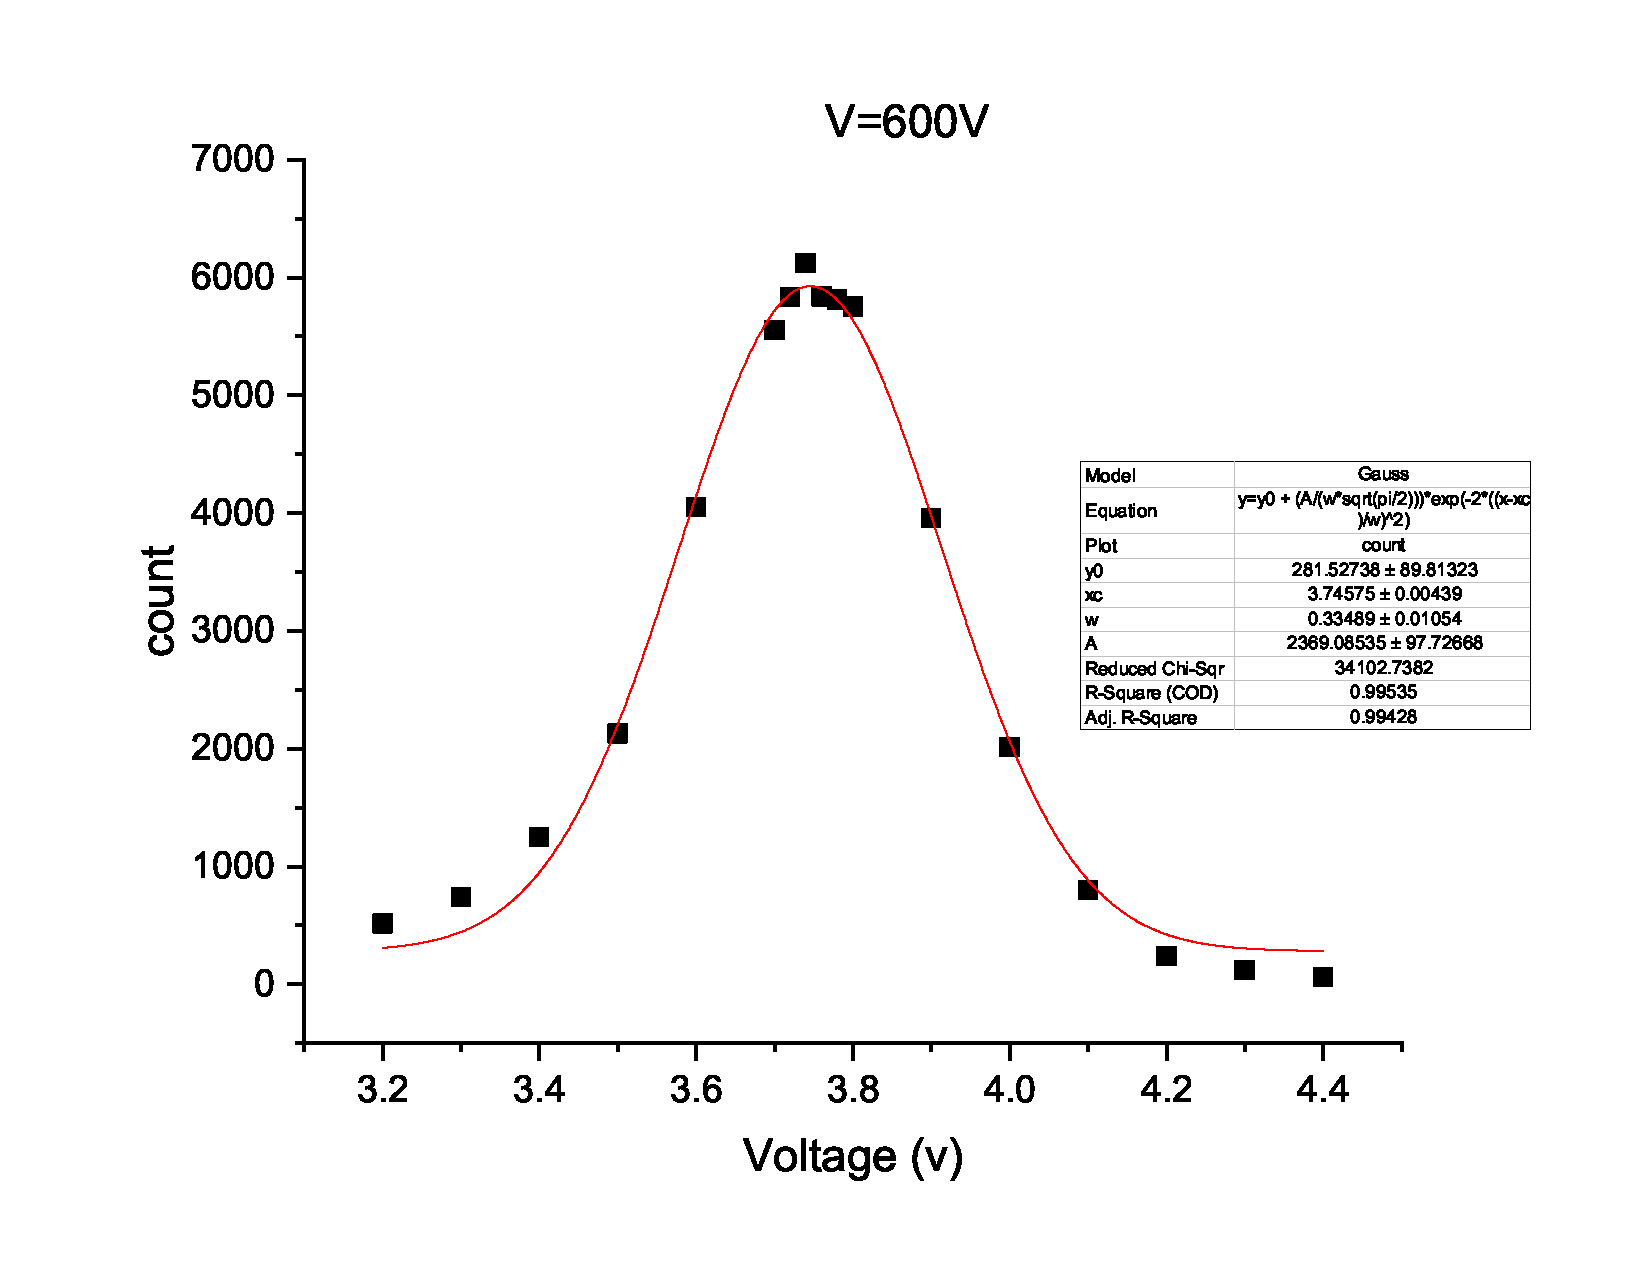
\includegraphics[width=90mm]{Graph3.eps}% Here is how to import EPS art
	% \caption{\label{fig:epsart}V vs counts}
	% \end{figure}
	% \subsubsection{\label{sec:level1}Operating voltage=500v}
	% table.4
	% \begin{table}[H]
    \centering
    \begin{tabular}{|c|c|c|c|c|}
        \hline
        Temperature & R       & c(pF) & C1     & $\epsilon$ \\ \hline
        $^{\circ}$C & K$\ohm$ & pF    & pF     & ~          \\ \hline
        50          & 1.111   & 1150  & 370.33 & 745.14     \\ \hline
        60          & 1.118   & 750   & 372.67 & 749.83     \\ \hline
        70          & 1.146   & 700   & 382.00 & 768.61     \\ \hline
        80          & 1.16    & 750   & 386.67 & 778.00     \\ \hline
        90          & 1.182   & 750   & 394.00 & 792.76     \\ \hline
        100         & 1.22    & 750   & 406.67 & 818.24     \\ \hline
        110         & 1.25    & 750   & 416.67 & 838.36     \\ \hline
        120         & 1.3     & 750   & 433.33 & 871.90     \\ \hline
        130         & 1.384   & 800   & 461.33 & 928.24     \\ \hline
        140         & 1.47    & 800   & 490.00 & 985.92     \\ \hline
        150         & 1.38    & 800   & 460.00 & 925.55     \\ \hline
        160         & 1.26    & 800   & 420.00 & 845.07     \\ \hline
        170         & 1.2     & 800   & 400.00 & 804.83     \\ \hline
        180         & 1.12    & 650   & 373.33 & 751.17     \\ \hline
    \end{tabular}
    \caption{observed capacitance value for $BaTiO_3$ at different temperature at 5kHz}
    \label{tab:4}
\end{table}
	% \begin{figure}[H]
	% \centering
	% \includegraphics[width=90mm]{Graph4.eps}% Here is how to import EPS art
	% \caption{\label{fig:epsart}V vs counts}
	% \end{figure}
	% \subsubsection{\label{sec:level1}Summary}
	% table.4
	% \begin{table}[H]
	\centering
	\resizebox{\columnwidth}{!}{%
	\begin{tabular}{|ccc|c|}
	\hline
	\multicolumn{1}{|c|}{$ne\times10^{-19}$} & \multicolumn{1}{c|}{ne divided by the lowest} & $n_{eff}$ & $e = \frac{ne}{n_{eff}}$   $(\times10^{-19})$ (c) \\ \hline
	\multicolumn{1}{|c|}{6.24} & \multicolumn{1}{c|}{1.52} & 2.00 & 3.12 \\ \hline
	\multicolumn{1}{|c|}{6.59} & \multicolumn{1}{c|}{1.61} & 2.00 & 3.30 \\ \hline
	\multicolumn{1}{|c|}{10.60} & \multicolumn{1}{c|}{2.58} & 3.00 & 3.53 \\ \hline
	\multicolumn{1}{|c|}{6.32} & \multicolumn{1}{c|}{1.54} & 2.00 & 3.16 \\ \hline
	\multicolumn{1}{|c|}{13.97} & \multicolumn{1}{c|}{3.40} & 3.00 & 4.66 \\ \hline
	\multicolumn{1}{|c|}{4.10} & \multicolumn{1}{c|}{1.00} & 1.00 & 4.10 \\ \hline
	\multicolumn{1}{|c|}{4.43} & \multicolumn{1}{c|}{1.08} & 1.00 & 4.43 \\ \hline
	\multicolumn{3}{|c|}{Average value of e} & 3.76 \\ \hline
	\multicolumn{3}{|c|}{$\delta e$ (standard   deviation)} & 0.63 \\ \hline
	\end{tabular}%
	}
	\caption{Dynamic Method find value of e}
	\label{tab:5}
\end{table}
	% \begin{figure}[H]
	% \centering
	% \includegraphics[width=90mm]{Graph5.eps}% Here is how to import EPS art
	% \caption{\label{fig:epsart}V vs counts}
	% \end{figure}\\
	% Thus from Fig.5 we have an operating voltage as 600v with a resolution of 10.11\%.
